\chapter{Evaluation}\label{chap:eval}

A user study was conducted to evaluate Replico's efficiency, effectiveness, and user-friendliness. The main goal was determining how easily users could communicate points of interest within the virtual environment using Replico. Secondary goals included assessing ease of use and overall user experience. The study aimed to answer four key research questions:

\begin{itemize}
    \item \textbf{RQ1}: How efficiently can users create a point of interest on a given object?
    \item \textbf{RQ2}: How effectively does Replico notify users when a point of interest is created?
    \item \textbf{RQ3}: How useful is the world-in-miniature metaphor for communicating points of interest? How useful is the representation of user locations on the replica for understanding intent? % 2nd part is inconclusive, users didn't use it :(
    \item \textbf{RQ4}: How user-friendly is Replico, and how much physical effort is required to use it? 
\end{itemize}

\section{Setup}

    % TODO: get computer specs

    The user study was conducted at FEUP, in the GIG laboratory in room I220. The setup included two VR-ready computers connected to a local network. Each computer had an HTC Vive Pro 2 headset and a VR controller for table tracking. Two touch surfaces -- a 32-inch infrared frame and a 47-inch capacitive Displax Skin Ultra touchscreen -- were placed on opposite tables within the central VR play space. Participants, in pairs, were seated in front of each touch surface with their backs facing each other, as shown in Figure \ref{fig:eval_setup}.

    \begin{figure}[h]
        \centering
        \includegraphics[width=1\linewidth]{figures/setup.png}
        \caption{Setup for the user study. In image (a) one participant is seated in front of the Displax Skin Ultra. In image (b) the participant is seated in front of the infrared touch frame.}
        \label{fig:eval_setup}
    \end{figure}

    One computer served as the host, while the other connected as a client. The setup process involved a starting screen where the moderator could select the IP address of the host computer. The roles of each computer did not change throughout the study to simplify the setup process and avoid confusion.

\section{Methodology}

    The study was conducted in pairs, with initial tasks performed individually and later tasks performed collaboratively. Each session consisted of three main parts: an introduction, a training session, and the main tasks. Each session lasted approximately 60 minutes. After each session, participants received a chocolate bar as a token of appreciation.

    Before the study began, participants were introduced briefly to the study's purpose and the Replico system. They then completed a consent form and a profiling questionnaire. Following this, they watched a video presentation explaining Replico's features, usage, and the tasks they would perform.

    During the training session, participants familiarized themselves with the system by experimenting with all of Replico's features. Once comfortable with the solo interactions, a set of points of interest and a simulated player were added to the environment, allowing users to practice acknowledging points of interest and joining the other user's table. After becoming comfortable with these interactions, they proceeded to the main tasks.

    The main tasks were performed using two different 3D models: a city and the Perseverance rover, described in Section \ref{sec:test_scenarios}. The order in which the models were used alternated between pairs to avoid bias. These tasks aimed to assess the efficiency and effectiveness of Replico's features, as described in Section \ref{sec:tasks}. Metrics for each task were collected as detailed in Section \ref{sec:evaluation_metrics}. Participants completed a questionnaire on the tasks they performed between each test scenario, described in Section \ref{sec:qualitative_data}.

    \subsection{Test Scenarios} \label{sec:test_scenarios}

        Three scenarios were used during the study, two for the main tasks, as shown in Figure \ref{fig:test_scenarios}. The first scenario, used for training, is a small dungeon tavern built with the free version of the KayKit Dungeon Remastered Pack from itch.io\footnote{\url{https://kaylousberg.itch.io/kaykit-dungeon-remastered}} and the Modular Asset Staging Tool (MAST) for Unity\footnote{\url{https://fertile-soil-productions.itch.io/mast}}. The second scenario is a city from Synty's POLYGON City Pack\footnote{\url{https://assetstore.unity.com/packages/3d/environments/urban/polygon-city-low-poly-3d-art-by-synty-95214}}, obtained through Unity's student plan. The third scenario features the Perseverance rover, obtained from NASA's 3D model repository\footnote{\url{https://nasa3d.arc.nasa.gov/detail/perseverance-glb}}, with the surrounding environment created using Unity's terrain tools and a tinted sand texture from Polyhaven\footnote{\url{https://polyhaven.com/a/sand_01}}.

        \begin{figure}[h]
            \centering
            \includegraphics[width=1\linewidth]{figures/test_scenarios.png}
            \caption{The three test scenarios used in the user study. From left to right: the dungeon tavern, the city, and the Perseverance rover.}
            \label{fig:test_scenarios}
        \end{figure}

        Two scenarios were selected for the main tasks to evaluate how well the approach works with different 3D models. The city model was chosen for its large, complex structure, allowing users to immerse themselves within it. The Perseverance rover model was selected for its smaller size but sufficient detail, enabling users to view the entire model at once without being part of it. The dungeon tavern was used for practice, providing a small, enclosed environment distinct from the main task scenarios.

        In all scenarios, the virtual world includes surrounding environment elements to provide context and a sense of scale. For example, the city is bordered by an ocean, the rover by the Martian surface, and the dungeon tavern by some of its walls. The WIM does not replicate these environmental elements, as they are not part of the primary scenario.

    \subsection{Tasks} \label{sec:tasks}

        Participants performed five main tasks during the study, using each of the two main scenarios. The first three tasks were done individually, while the last two were collaborative. Each task evaluated different aspects of Replico's features and user experience. The tasks are as follows:

        \begin{itemize}
            \item \textbf{Task 1}: Create a point of interest on six different predefined objects in the scene. This task evaluates how efficiently users can create points of interest.
            \item \textbf{Task 2}: Acknowledge five out of twelve predefined points of interest created by a simulated user. This task assesses how effectively Replico notifies users of new points of interest.
            \item \textbf{Task 3}: Teleport to four different predefined zones and orient themselves to face a specific object. This task measures how well users can navigate the environment using Replico.
            \item \textbf{Task 4 \& 5}: One user must show another user a specific object in the scene without verbal communication. The other user then verbally confirms the object they believe the first user is referring to. Once confirmed, the roles are reversed, and the process is repeated with a different object. This task evaluates how well users can communicate points of interest using Replico
        \end{itemize}

        Between each task, the environment was reset to its initial state. This meant that any points of interest created during the previous task were removed, and participants were placed back at their starting positions. This was done to ensure that each task was performed under the same conditions for all participants.

        In the first task, the predefined objects were chosen with different sizes and at various heights, visible in Figure \ref{fig:task_01}. The goal was to evaluate how efficiently users could create points of interest, not to test their ability to identify objects. To draw attention to them, these objects glowed with an expanding and contracting effect in the WIM. They increased in size and changed their outline color from white to green when the balloon intersected with them. Creating a point of interest during this state allowed users to progress to the next object. The objects appeared one at a time, immediately after the user created a point of interest on the previous object. The order in which the objects appeared was consistent for all participants.

        \begin{figure}[h!]
            \centering
            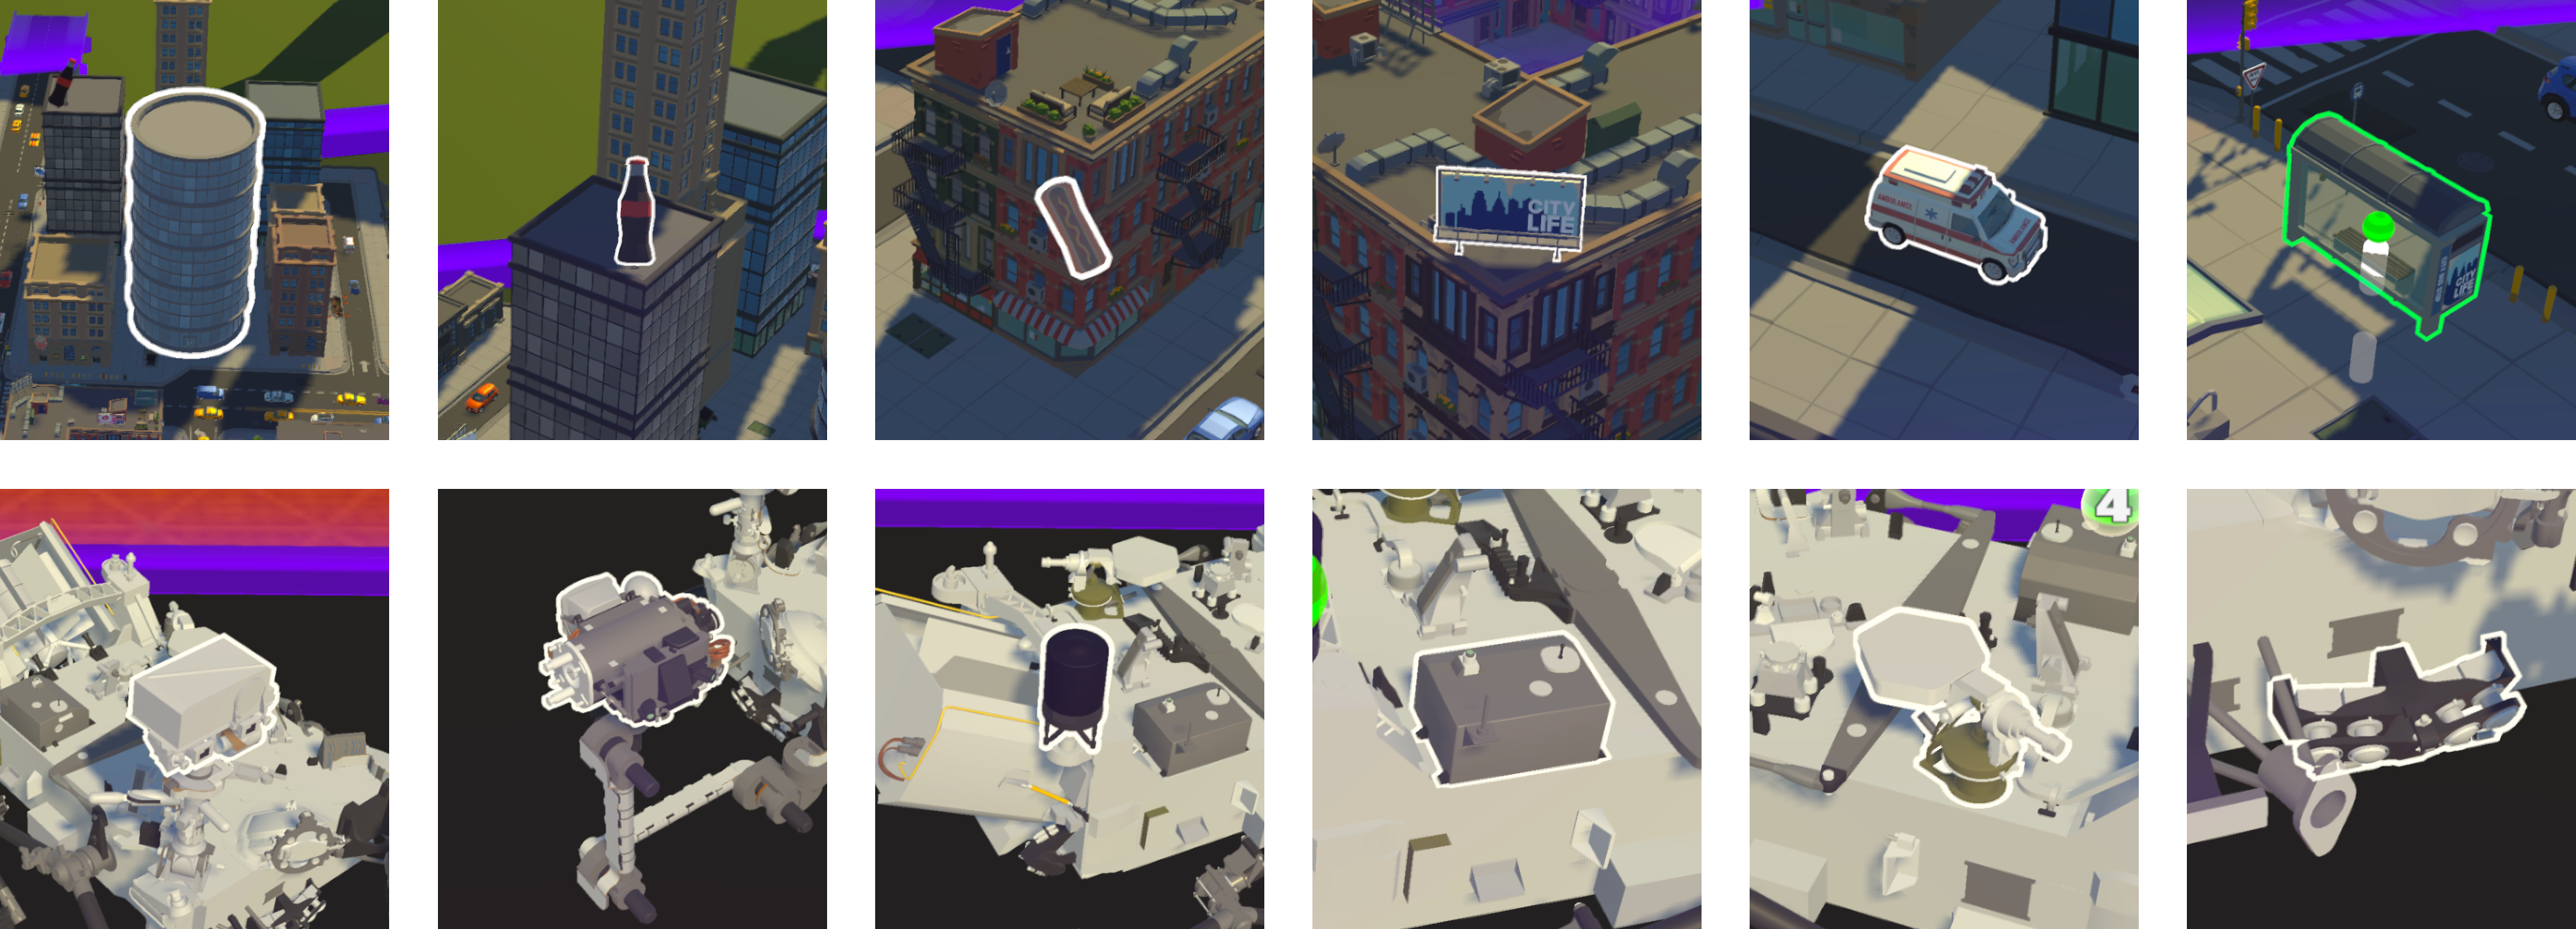
\includegraphics[width=1\linewidth]{figures/task_01.png}
            \caption{The six predefined objects used in Task 1 for each scenario. They are ordered from left to right, with the top row showing the objects in the city scenario while the bottom row shows the objects in the Perseverance rover scenario. The top-right image shows the green outline effect that appears when the balloon intersects with the object.}
            \label{fig:task_01}
        \end{figure}

        In the second task, the predefined points of interest were placed around the environment simultaneously, as shown in Figure \ref{fig:task_02}. The goal was to evaluate how effectively Replico notifies users of new points of interest and helps distinguish acknowledged from unacknowledged points of interest. The task was complete when the user acknowledged the five unacknowledged points of interest. Participants could acknowledge the points of interest in any order.

        \begin{figure}[h!]
            \centering
            \includegraphics[width=1\linewidth]{figures/task_02.png}
            \caption{The created points of interest in Task 2. Image (a) shows the points of interest in the city scenario, while image (b) shows the points of interest in the Perseverance rover scenario.}
            \label{fig:task_02}
        \end{figure}

        In the third task, participants navigated through four predefined zones in the environment, as shown in Figure \ref{fig:task_03}. The goal was to assess how well users could navigate using Replico. Participants were instructed to teleport to each zone and orient themselves to face a specific object. Zones changed color from white to green when the balloon intersected with them, and the object's glow effect also changed from white to green when the user was correctly oriented. The moderator advanced the task manually, allowing participants to take their time exploring the environment. The sequence of zones was the same for all participants.

        \begin{figure}[h]
            \centering
            \includegraphics[width=1\linewidth]{figures/task_03.png}
            \caption{The four predefined zones used in Task 3 for each scenario. They are ordered from left to right, with the top row showing the zones in the city scenario while the bottom row shows the zones in the Perseverance rover scenario.}
            \label{fig:task_03}
        \end{figure}

        In the fourth and fifth tasks, participants communicated objects of interest without verbal communication. Figure \ref{fig:task_04} shows the objects used in these tasks. The goal was to assess how effectively users could communicate using Replico. The selected objects were small and difficult to identify from a distance, encouraging the use of the WIM, points of interest, and teleportation for effective communication. For the Perseverance rover model, since most people are unfamiliar with its components, the objects chosen were a small hidden star and a small hidden heart.

        \begin{figure}[h]
            \centering
            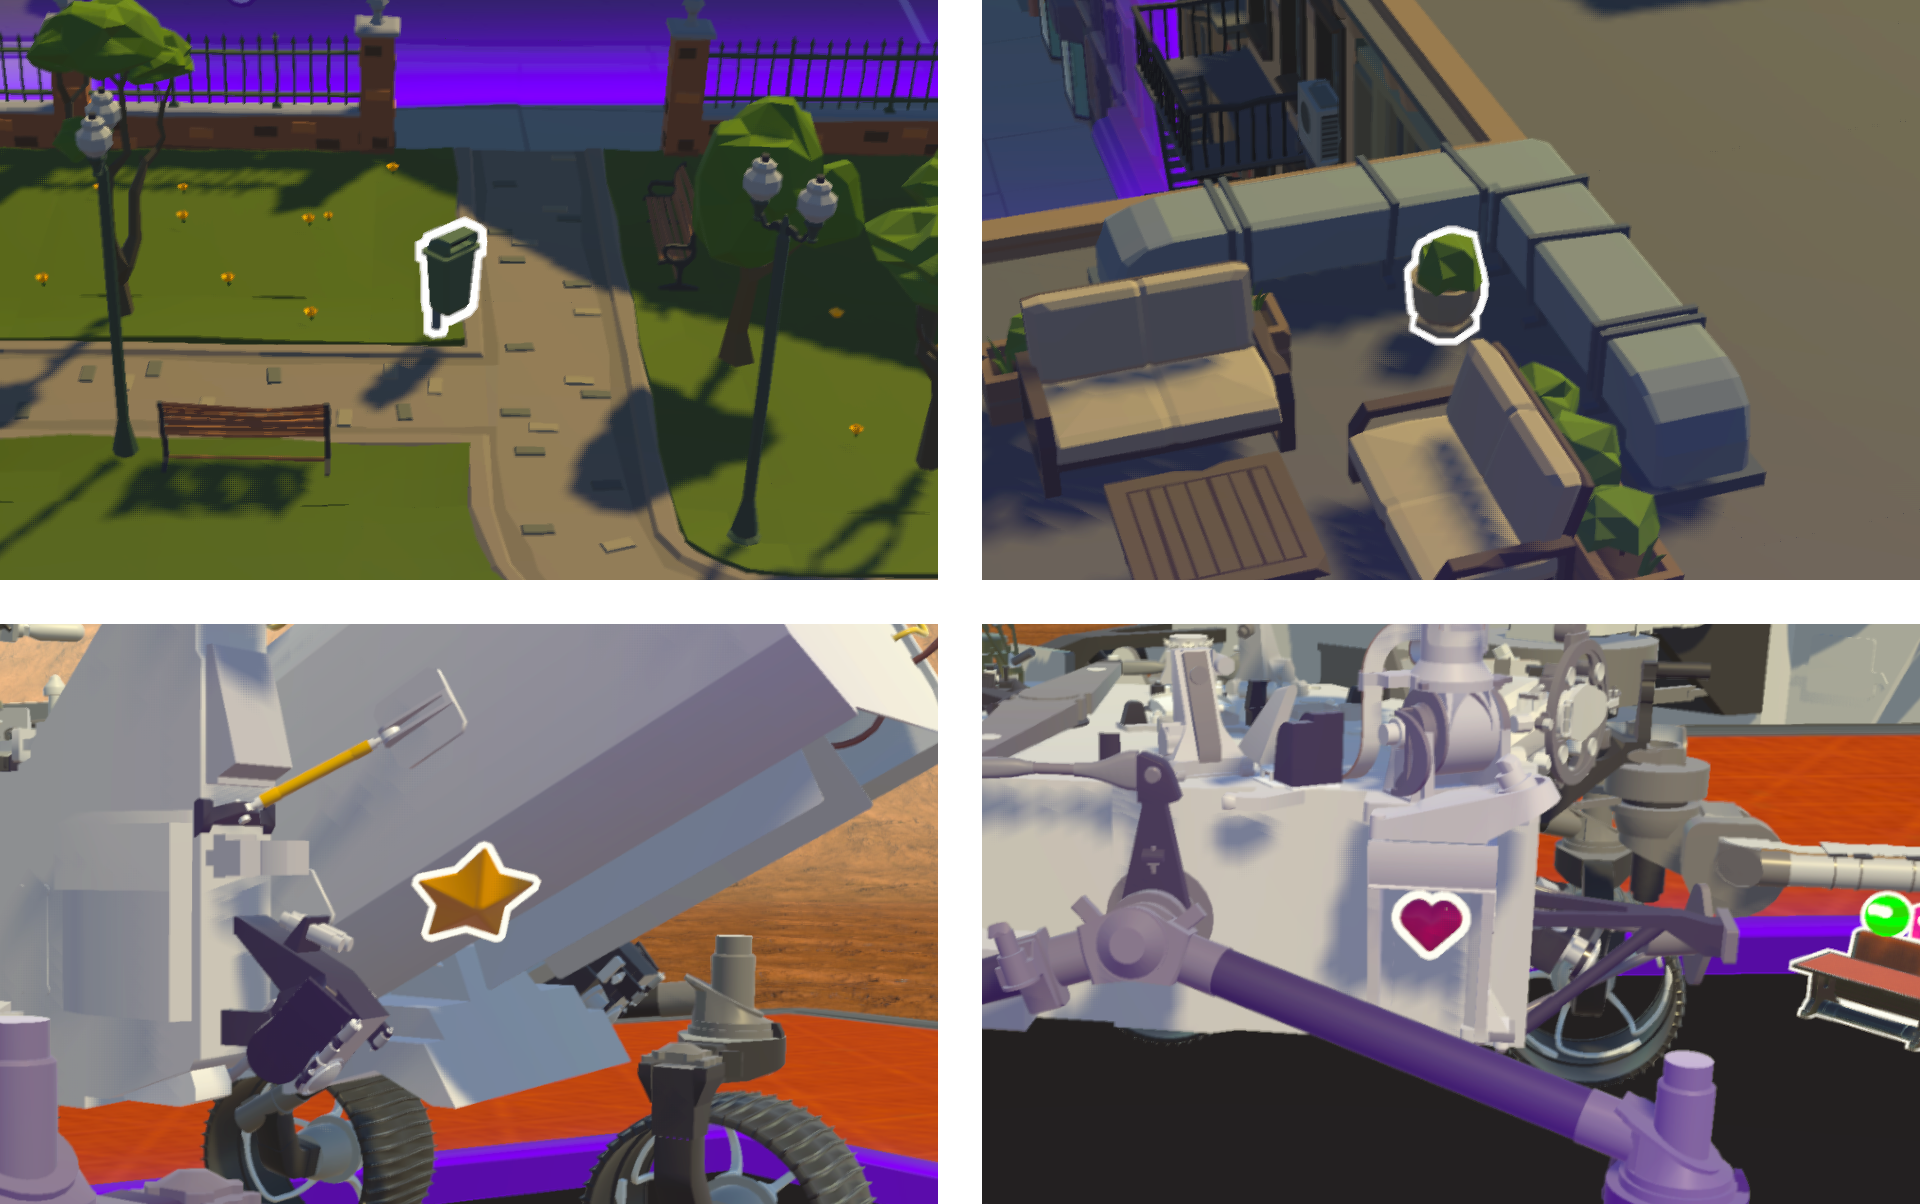
\includegraphics[width=1\linewidth]{figures/task_04.png}
            \caption{The objects used in Tasks 4 and 5 for each scenario. The top row shows the objects in the city scenario, while the bottom row shows the objects in the Perseverance rover scenario.}
            \label{fig:task_04}
        \end{figure}


    \subsection{Metrics} \label{sec:evaluation_metrics}

        During each task, several metrics were collected to evaluate the efficiency and effectiveness of Replico's features. These metrics, recorded automatically by the system, included the time in seconds taken to complete the task, the number of successful task steps, time spent transforming the replica, time spent in vertical transformation, and time spent in balloon selection. Additionally, the system tracked the number of times the transform gesture was detected (on entering \lstinline{TransformReplicaState}), the number of times vertical transform was detected (on entering \lstinline{TransformReplicaVerticalState}), and the number of times the balloon selection gesture was detected (on entering \lstinline{BalloonSelectionInitialState}). It also recorded the number of points of interest created, deleted, and acknowledged, the number of teleportations, the number of table joins, the number of touches on the touch surface, the cumulative sum of finger movement in pixels, the cumulative sum of head rotation in angles, cumulative head translation in meters, cumulative sum of replica rotation in angles, cumulative sum of replica translation in meters, and cumulative sum of replica scaling in meters.

        The time taken to complete each task was measured from the start to the end of the task. In Task 3, while the participant waited for the moderator to advance to the next zone, all metrics were paused. The number of successful task steps was the number of steps completed correctly by the user. For example, in Task 1, a successful step was creating a point of interest on a predefined object. In Task 2, a successful step was acknowledging a point of interest. In Task 3, a successful step was teleporting to a zone and orienting oneself to face a specific object. In Tasks 4 and 5, it referred to the number of guesses until the correct object was identified.

        Additionally, for each frame that showed a change, data was collected and timestamped. This included finger data, replica transform data, and head transform data
    
    \subsection{Qualitative Data} \label{sec:qualitative_data}

        After each test scenario, participants completed a questionnaire to provide qualitative feedback on their experience. The questionnaire included six questions from the NASA Task Load Index (NASA-TLX) \cite{hart1988development} for each task, along with three additional questions at the end of the questionnaire, each rated on a 5-point Likert scale. The NASA-TLX questions were:

        \begin{itemize}
            \item How mentally demanding was the task?
            \item How physically demanding was the task?
            \item How hurried or rushed was the pace of the task?
            \item How successful were you in accomplishing what you were asked to do?
            \item How hard did you have to work to accomplish your level of performance?
            \item How insecure, discouraged, irritated, stressed, and annoyed were you?
        \end{itemize}

        The final three questions were:

        \begin{itemize}
            \item How nauseous did you feel during the task?
            \item How useful was the world-in-miniature metaphor for communicating points of interest?
            \item How useful was the representation of user locations on the replica for understanding intent?
        \end{itemize}

        Participants were also encouraged to provide additional comments or suggestions for improvement. The aim was to gather feedback on the user experience and identify areas for improvement in the system.

\section{Participants}

    A total of 20 participants, forming 10 pairs, took part in the study. Among them, eleven were male, and 9 were female. Most participants, 19, were aged between 21 and 30 years old, with one participant aged between 31 and 40. 19 participants were right-handed, and one was left-handed. 17 participants were students, of whom six also worked, while three were exclusively workers. 15 participants had completed a bachelor's degree, two had a master's degree, and three had a high school diploma. Regarding VR experience, 11 had used VR once before, three had used it in the past year, one used it frequently, and five had never used VR before.

\section{Results}

    The results of the user study are presented in this section. Two samples were collected for each task metric, one for each test scenario. For each metric, appropriate statistical tests were performed to determine the significance of the results. The significance level was set to the conventional alpha-value of 5\%.


    \subsection{Metrics}

        % todo: what metrics are we going to show?
        
        Using descriptive data analysis, outliers were identified and removed from the dataset. The data was then analysed with the Shapiro-Wilk \cite{shapiroAnalysisVarianceTest1965} test to determine if it followed a normal distribution. Because the analysis is testing two related samples, either the paired t-test or the Wilcoxon signed-rank test \cite{wilcoxonIndividualComparisonsRanking1945} was used to determine if the differences between the samples were statistically significant. The paired t-test was used when the data followed a normal distribution, while the Wilcoxon signed-rank test was used when the data did not follow a normal distribution.

        \subsubsection{Task Completion Time}

            % task1city follows a normal distribution (p = .128)
            % task2city follows a normal distribution (p = .268)
            % task3city does not follow a normal distribution (p=.004) --!
            % task4city does not follow a normal distribution (p=.005)
            % task5city does not follow a normal distribution (p=.002)
            % task1rover follows a normal distribution (p = .064)
            % task2rover follows a normal distribution (p = .735)
            % task3rover follows a normal distribution (p = .580) -- !
            % task4rover does not follow a normal distribution (p=.026)
            % task5rover does not follow a normal distribution (p=.012)

            \begin{figure}[h]
                \centering
                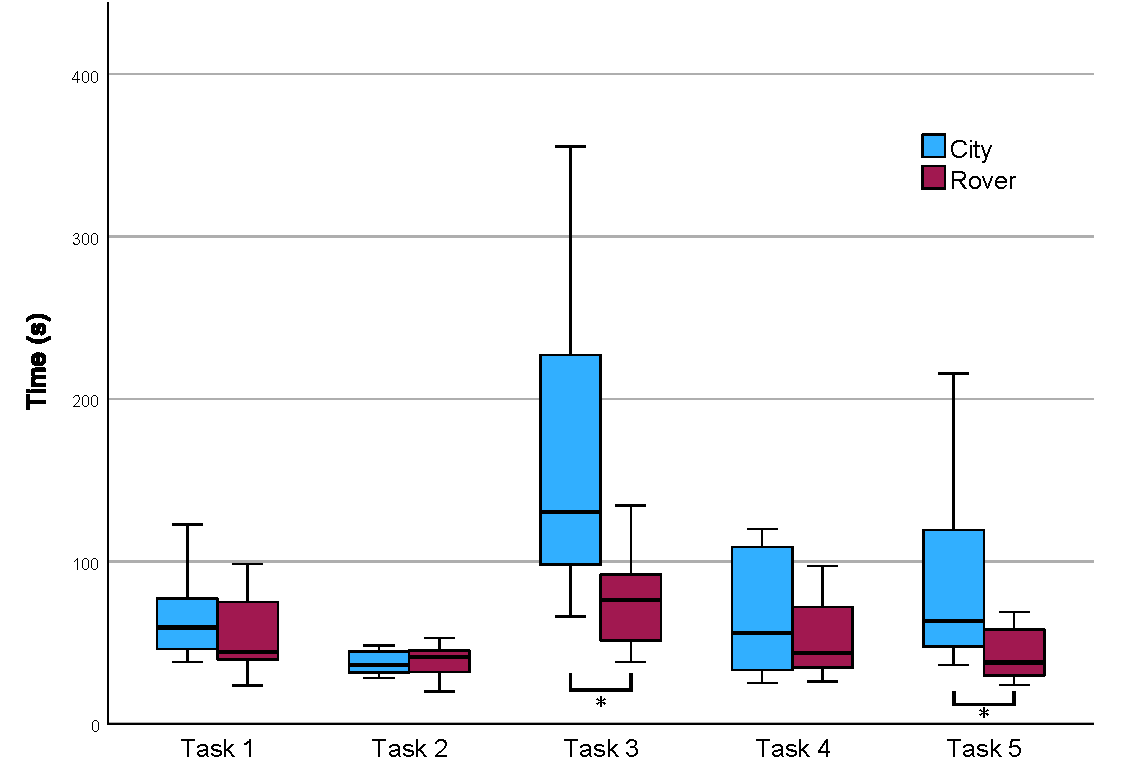
\includegraphics[width=1\linewidth]{figures/task_time_graph.pdf}
                \caption{Box-plot of the time taken to complete each task for each scenario.}
                \label{fig:task_time}
            \end{figure}

            % task1 using paired t-test
                % t(15) = 1.440, p =.172
                % no significant difference between the time taken to complete Task 1 in the city and rover scenarios
            % task2 using paired t-test
                % t(11) = .134, p =.896
                % no significant difference between the time taken to complete Task 2 in the city and rover scenarios
            % task3 using Wilcoxon signed-rank test
                % Z = -3.248, p=.001
                % significant difference between the time taken to complete Task 3 in the city and rover scenarios: participants took longer to complete the task in the city scenario
                % why? i think its because it was harder to find the objects in the city scenario, also the zones were more spread out, and smaller. People had a hard time zooming in on the objects, and instead tried teleporting with a small zoom, which was not effective
            % task 4 using Wilcoxon signed-rank test
                % Z = -1,415, p=.157
                % no significant difference between the time taken to complete Task 4 in the city and rover scenarios
                % good, this means that the difficulty of the objects was similar in both scenarios
            % task 5 using Wilcoxon signed-rank test
                % Z = -3.154, p=.002
                % significant difference between the time taken to complete Task 5 in the city and rover scenarios: participants took longer to complete the task in the city scenario
                % task 5 in the city had a really small object, in the midst of a lot of other objects, which made it harder to find. The rover objects sometimes people would find them by accident, which made it easier to complete the task. Also, the points of interest would obscure the objects, making it harder to find them, because participants didnt teleport to the objects, they would just zoom in on them, which was not effective. Some participants had issues with depth perception, so it was hard for them to place the points of interest.

        \subsubsection{Active Time}

            % task1city p = .042: does not follow a normal distribution
            % task2city p = .572: follows a normal distribution
            % task3city p=.005: does not follow a normal distribution
            % task4seekcity p=.285: follows a normal distribution
            % task4showcity p=.252: follows a normal distribution
            % task5seekcity p=.079: follows a normal distribution
            % task5showcity p=.177: follows a normal distribution
            % task1rover p = .068: follows a normal distribution
            % task2rover p = .802: follows a normal distribution
            % task3rover p = .209: follows a normal distribution
            % task4seekrover p =.241: follows a normal distribution
            % task4showrover p =.611: follows a normal distribution
            % task5seekrover p =.153: follows a normal distribution
            % task5showrover p =.024: does not follow a normal distribution

            \begin{figure}[h]
                \centering
                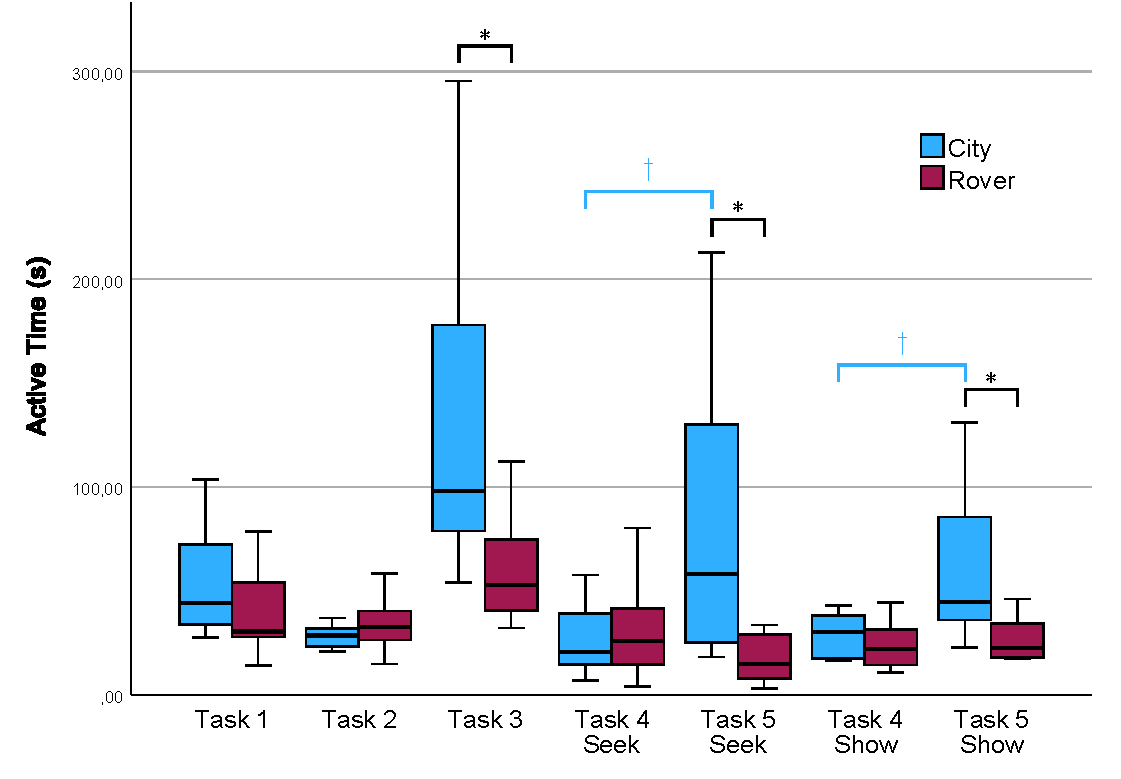
\includegraphics[width=1\linewidth]{figures/active_time_graph.pdf}
                \caption{Box-plot of the active time for each task for each scenario.}
                \label{fig:active_time}
            \end{figure}

            % task1 using Wilcoxon signed-rank test
                % Z = -1.913, p =.056
                % no significant difference between the active time in Task 1 in the city and rover scenarios
            % task2 using paired t-test
                % t(13) = -1.431, p = .178
                % no significant difference between the active time in Task 2 in the city and rover scenarios
            % task3 using Wilcoxon signed-rank test
                % Z = -3.051, p=.002
                % significant difference between the active time in Task 3 in the city and rover scenarios: participants spent more time active in the city scenario
            % task4seek using paired t-test
                % t(9) = -.305, p =.767
                % no significant difference between the active time in Task 4 in the city and rover scenarios
            % task4show using paired t-test
                % t(7) = .434, p =.677
                % no significant difference between the active time in Task 4 in the city and rover scenarios
            % task5seek using paired t-test
                % t(9) = 2.929, p =.017
                % significant difference between the active time in Task 5 in the city and rover scenarios: participants spent more time active in the city scenario
                % why? after the other person made a point of interest, the other person would spend a lot of time looking for the object, which would increase the active time
            % task5show using Wilcoxon signed-rank test
                % Z = -2.521, p=.012
                % significant difference between the active time in Task 5 in the city and rover scenarios: participants spent more time active in the city scenario


        \subsubsection{Finger Movement}

            % task1city p = .455: follows a normal distribution
            % task2city p = .2: follows a normal distribution
            % task3city p =.045: does not follow a normal distribution
            % task4seekCity p =.409: follows a normal distribution
            % task4showCity p =.479: follows a normal distribution
            % task5seekCity p =.621: follows a normal distribution
            % task5showCity p =.018: does not follow a normal distribution
            % task1rover p = .323: follows a normal distribution
            % task2rover p = .801: follows a normal distribution
            % task3rover p = .255: follows a normal distribution
            % task4seekRover p = .358: follows a normal distribution
            % task4showRover p = .582: follows a normal distribution
            % task5seekRover p = .177: follows a normal distribution
            % task5showRover p = .921: follows a normal distribution

            \begin{figure}[h]
                \centering
                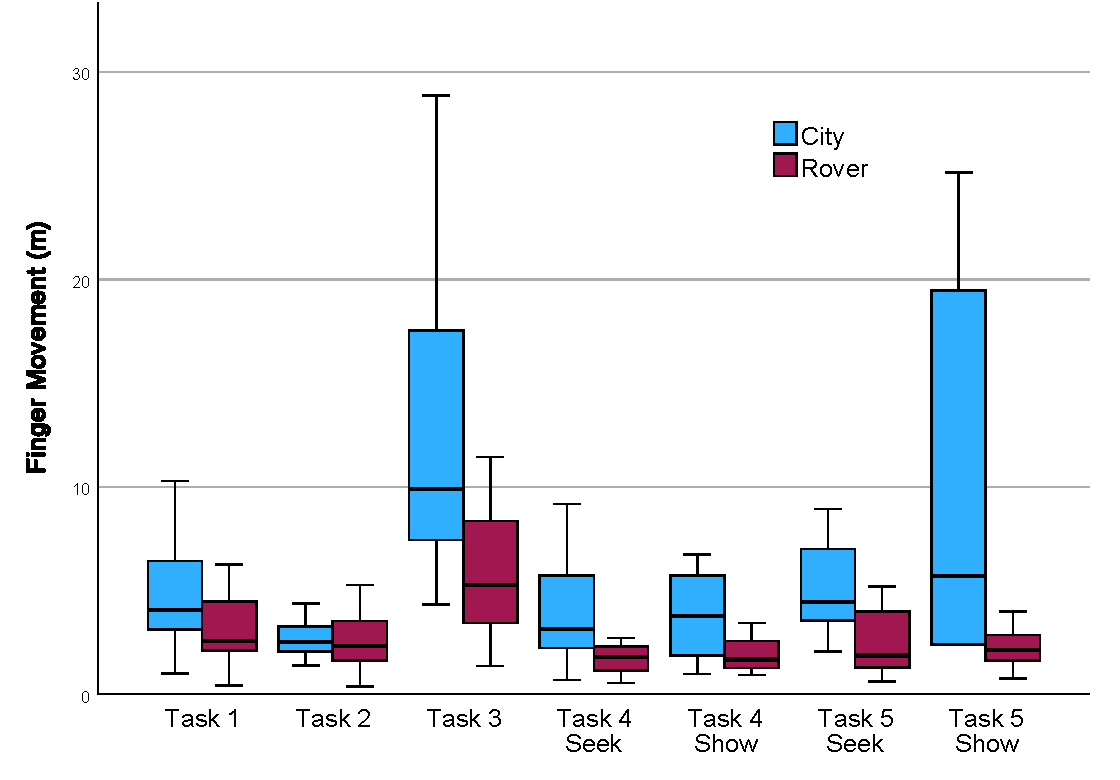
\includegraphics[width=1\linewidth]{figures/finger_movement_graph.pdf}
                \caption{Box-plot of the cumulative sum of finger movement in meters for each task for each scenario.}
                \label{fig:finger_movement}
            \end{figure}

            % task1 using paired t-test
                % t(15) = 2.976, p =.010
                % significant difference between the cumulative sum of finger movement in Task 1 in the city and rover scenarios: participants moved their fingers more in the city scenario
                % why? objects more spread out, harder to find, more zooming in and out, interesting metric to explore: zooming amount?
            % task2 using paired t-test
                % t(16) = 1.030, p =.320
                % no significant difference between the cumulative sum of finger movement in Task 2 in the city and rover scenarios
            % task3 using Wilcoxon signed-rank test
                % Z = -3.285, p=.001
                % significant difference between the cumulative sum of finger movement in Task 3 in the city and rover scenarios: participants moved their fingers more in the city scenario
            % task4seek using paired t-test
                % t(8) = 1.765, p =.121
                % no significant difference between the cumulative sum of finger movement in Task 4 in the city and rover scenarios
            % task4show using paired t-test
                % t(8) = 2.059, p =.078
                % no significant difference between the cumulative sum of finger movement in Task 4 in the city and rover scenarios
            % task5seek using paired t-test
                % t(8) = 3.221, p =.015
                % significant difference between the cumulative sum of finger movement in Task 5 in the city and rover scenarios: participants moved their fingers more in the city scenario
            % task5show using Wilcoxon signed-rank test
                % Z = -2.380, p=.017
                % significant difference between the cumulative sum of finger movement in Task 5 in the city and rover scenarios: participants moved their fingers more in the city scenario

        \subsubsection{Point of Interest Creation}

            % analysing because i noticed people were creating a lot of points of interest on accident

        \subsubsection{Replica Translation}

        \subsubsection{Replica Scale}

    \subsection{Qualitative Data}

        The results obtained from the questionnaires are discrete, ordinal data, as opposed to the continuous data obtained from the metrics. As such, the Wilcoxon signed-rank test was used to determine if there were significant differences between the responses for each question in each scenario.

        For the first task, Table \ref{tab:analysis_qualitative_1} shows the results. There were no significant differences between the city and rover scenarios for any of the questions. This suggests that the task load was similar in both scenarios. Participants didn't find the tasks mentally or physically demanding, nor did they feel rushed or insecure. They also felt successful in accomplishing what they were asked to do and felt lower-to-moderate effort was required to achieve their level of performance.
       
        \begin{table}[h!]
            \caption{Median (IQR), and Wilcoxon Signed Ranks test results for each of the NASA-TLX questions for the first task in each scenario.}
            \begin{tabularx}{1\textwidth}{X l l l}
                \hline
                \multirow{2}{*}{Question} & \multicolumn{2}{c}{Median (IQR)} & \multirow{2}{*}{Wilcoxon Signed Ranks} \\
                \cline{2-3}
                & \makecell{City} & \makecell{Rover} &  \\
                \hline
                \hline
                How mentally demanding was the task? & 2 (1) & 1 (1) & $Z = -0.977,\ p = 0.329$ \\
                How physically demanding was the task? & 1 (1) & 1 (0) & $Z = -1.633,\ p = 0.102$  \\
                How hurried or rushed was the pace of the task? & 2 (1.75) & 1 (2) & $Z = -1.578,\ p = 0.115$\\
                How successful were you in accomplishing what you were asked to do? & 5 (1) & 5 (0.75) & $Z = -1.100,\ p = 0.271$ \\
                How hard did you have to work to accomplish your level of performance? & 2 (1.75) & 2 (2) & $Z = -0.844,\ p = 0.399$ \\
                How insecure, discouraged, irritated, stressed, and annoyed were you? & 1 (0) & 1 (0) & $Z = 0.000,\ p = 1.000$ \\
            \end{tabularx}
            \label{tab:analysis_qualitative_1}
        \end{table}
 
        For the second task, Table \ref{tab:analysis_qualitative_2} shows the results. The city scenario was found to be statistically significantly more physically demanding than the rover scenario

        \begin{table}[h!]
            \caption{Median (IQR), and Wilcoxon Signed Ranks test results for each of the NASA-TLX questions for the second task in each scenario.}
            \begin{tabularx}{1\textwidth}{X l l l}
                \hline
                \multirow{2}{*}{Question} & \multicolumn{2}{c}{Median (IQR)} & \multirow{2}{*}{Wilcoxon Signed Ranks} \\
                \cline{2-3}
                & \makecell{City} & \makecell{Rover} &  \\
                \hline
                \hline
                How mentally demanding was the task? & 2 (1) & 1 (1) & $Z = -1.311,\ p = 0.190$  \\
                How physically demanding was the task? $\ast$ & 1 (1) & 1 (0) & $Z = -2.000,\ p = 0.046$ \\
                How hurried or rushed was the pace of the task? & 2 (1.75) & 1.5 (1) & $Z = -0.905,\ p = 0.366$ \\
                How successful were you in accomplishing what you were asked to do? & 5 (1) & 4.5 (1) & $Z = -0.378,\ p = 0.705$ \\
                How hard did you have to work to accomplish your level of performance? $\ast$ & 2 (1.75) & 1.5 (1) & $Z = -2.055,\ p = 0.040$ \\
                How insecure, discouraged, irritated, stressed, and annoyed were you? $\ast$ & 1 (0.25) & 1 (0) & $Z = -2.000,\ p = 0.046$ \\
            \end{tabularx}

            \label{tab:analysis_qualitative_2}
        \end{table} 

        \begin{table}[h!]
            \caption{Median (IQR), and Wilcoxon Signed Ranks test results for each of the NASA-TLX questions for the third task in each scenario.}
            \begin{tabularx}{1\textwidth}{X l l l}
                \hline
                \multirow{2}{*}{Question} & \multicolumn{2}{c}{Median (IQR)} & \multirow{2}{*}{Wilcoxon Signed Ranks} \\
                \cline{2-3}
                & \makecell{City} & \makecell{Rover} &  \\
                \hline
                \hline
                How mentally demanding was the task? & 2 (1) & 2 (2) & $Z = -0.819,\ p = 0.413$ \\
                How physically demanding was the task? & 2 (2) & 1 (1) & $Z = -1.613,\ p = 0.107$ \\
                How hurried or rushed was the pace of the task? & 2 (2) & 1 (1) & $Z = -1.394,\ p = 0.163$ \\
                How successful were you in accomplishing what you were asked to do? & 4 (1) & 4.5 (1) & $Z = 0.000,\ p = 1.000$ \\
                How hard did you have to work to accomplish your level of performance? & 3 (2) & 2 (2.5) & $Z = -1.279,\ p = 0.201$ \\
                How insecure, discouraged, irritated, stressed, and annoyed were you? & 1 (1) & 1 (0) & $Z = -1.633,\ p = 0.102$ \\
            \end{tabularx}

            \label{tab:analysis_qualitative_3}
        \end{table} 

        \begin{table}[h!]
            \caption{Median (IQR), and Wilcoxon Signed Ranks test results for each of the NASA-TLX questions for the fourth task in each scenario.}
            \begin{tabularx}{1\textwidth}{X l l l}
                \hline
                \multirow{2}{*}{Question} & \multicolumn{2}{c}{Median (IQR)} & \multirow{2}{*}{Wilcoxon Signed Ranks} \\
                \cline{2-3}
                & \makecell{City} & \makecell{Rover} &  \\
                \hline
                \hline
                How mentally demanding was the task? $\ast$ & 2 (1) & 2 (1) & $Z = -2.144,\ p = 0.032$ \\
                How physically demanding was the task? $\ast$ & 2 (1) & 1 (0.75) & $Z = -2.111,\ p = 0.035$\\
                How hurried or rushed was the pace of the task? & 2 (1.75) & 1.5 (2) & $Z = -1.604,\ p = 0.109$ \\
                How successful were you in accomplishing what you were asked to do? $\ast$ & 4 (1) & 5 (0) & $Z = -2.919,\ p = 0.004$ \\
                How hard did you have to work to accomplish your level of performance? & 2 (1) & 1 (1.75) & $Z = -1.489,\ p = 0.137$ \\
                How insecure, discouraged, irritated, stressed, and annoyed were you? & 1 (1) & 1 (0) & $Z = -1.890,\ p = 0.059$ \\
            \end{tabularx}

            \label{tab:analysis_qualitative_4}
        \end{table} 

        \begin{table}[h!]
            \caption{Median (IQR), and Wilcoxon Signed Ranks test results for each of the general evaluation questions in each scenario.}
            \begin{tabularx}{1\textwidth}{X l l l}
                \hline
                \multirow{2}{*}{Question} & \multicolumn{2}{c}{Median (IQR)} & \multirow{2}{*}{Wilcoxon Signed Ranks} \\
                \cline{2-3}
                & \makecell{City} & \makecell{Rover} &  \\
                \hline
                \hline
                How nauseous did you feel during the task? & 1 (0) & 1 (0) & $Z = 0.000,\ p = 1.000$ \\
                How useful was the world-in-miniature metaphor for communicating points of interest? & 5 (0.75) & 5 (0) & $Z = -1.732,\ p = 0.083$ \\
                How useful was the representation of user locations on the replica for understanding intent? & 4 (1) & 5 (1) & $Z = -0.632,\ p = 0.527$ \\
            \end{tabularx}
            \label{tab:analysis_qualitative_g}
        \end{table}

    \subsection{Observations}

% do speak about how the frame being too sensitive to resting arms impacted the results
    % infrared table: because it does not track fingers on touch, but instead using infrared, it would pick up extra fingers if the user didn't lift their hands high enough, or fingers came too close together. This led to many points of interest created on accident
        % it also had a relatively low resolution, which made it hard to select small objects. This could be mitigated by scaling the replica, but it was not intuitive for some users to do so.
    % displax table: had some issue with losing fingers when moving them, which would sometimes cancel gestures. It also required fingers to be more spread out or else it would consider them as one finger. Adittionaly, because the table was so light-reflective, if the user approached the table, the headset tracking would start jittering.
        % even with the mitigation of not terminating the gesture for some time after the finger was lost, it was still an issue as it would sometimes switch fingers from on hand to the other, changing the balloon's position.
% teleport destination did not match the user's head, but instead the bottom of the table, which was confusing for some users.
% vertical transform rarely used
% depth perception issues
    % the limits of the table were not clear to some users because of this. This is also because the limit effect is not perfect, it has the same direction as the user's view point, instead of outwards or inwards from the limits of the table.
    % it was very discouraging for some users.
% headset tracking issues
% people forgetting how to teleport
% teleporting hard to understand
    % especially in regards to long press, and the rotation of the balloon
% many points of interest created by accident
% points of interest obscuring objects
% no easy way to know your color
% task 3 was confusing for some people because they didn't know what they were supposed to do. They either thought you only had to teleport to the zones, or they didn't know they had to orient themselves to face the object.
    % another issue was that if you created a point of interest by accident near a zone, it would obscure the zone. Because the system prioritizes the zones over the points of interest, users usually had a hard time deleting those points of interest, and so they couldnt see the zone and if they were inside the zone correctly (see it change to green)
% usually the second scenario would always be better than the first, because people would get used to the system.
% would be cool to see exactly where someone is looking at, like a raycast from the eyes
% -- positives --
% users liked that they could see each other.
% users found balloon selection easy to use, and intuitive

    \subsection{Discussion}

    \section{Summary}
